\documentclass{standalone}
\usepackage{tikz, fixmath}
\usetikzlibrary{quotes,angles, positioning}
\begin{document}
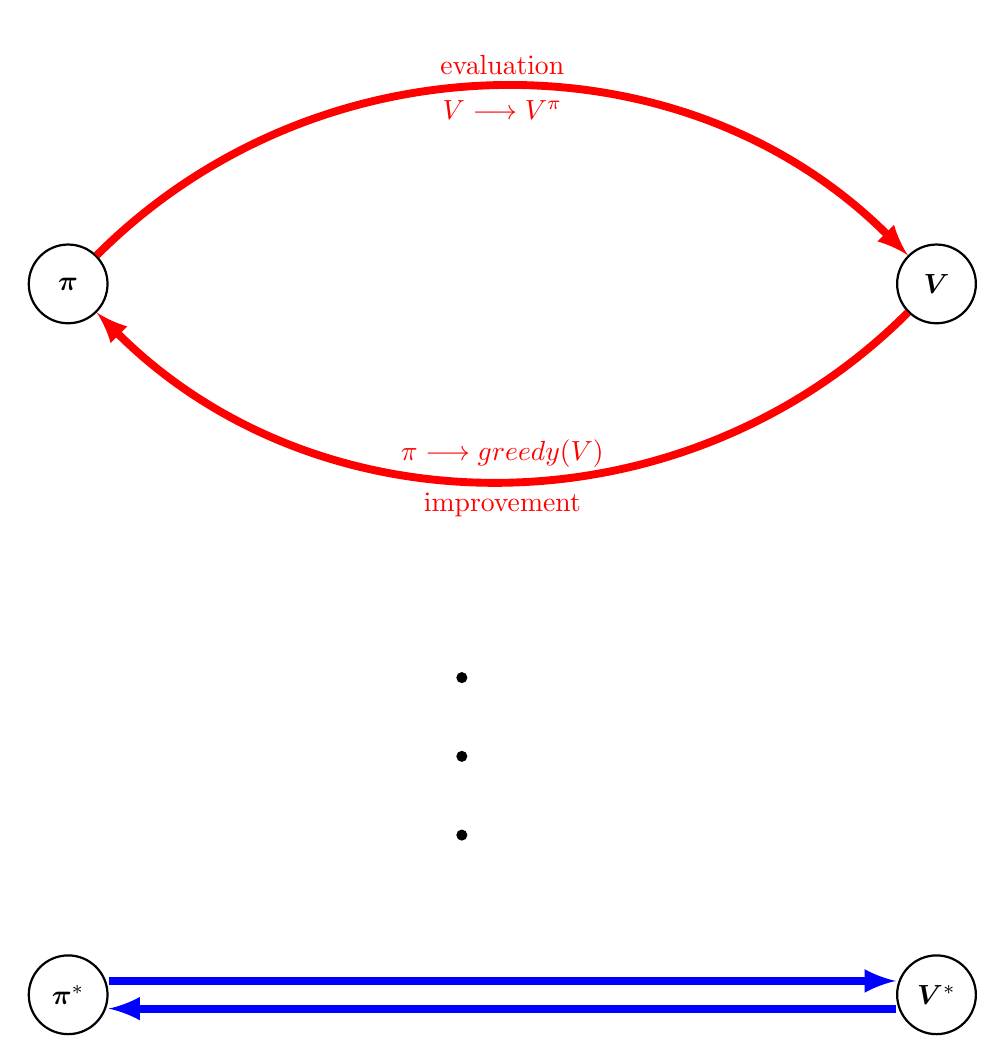
\begin{tikzpicture}[%
    ,>=latex
    ,latent/.style={%
        ,circle
        ,draw
        ,thick
        ,minimum size=10mm
        }
    ]   
    \node [latent] (pi) at (0,0) {$\mathbold{ \pi}$};
    \node [latent] (LV2) [right =10 cm of pi]  {$\mathbold{V}$};
    \draw [->, bend angle=45, bend left, line width=1mm, red]  (pi) to node[below] {$V \longrightarrow V^\pi$} node[above] {evaluation} (LV2);
    \draw [<-, bend angle=45, bend right, line width=1mm, red]  (pi) to node[below] {improvement} node[above] {$\pi \longrightarrow greedy(V)$} (LV2);

    \foreach \i in {-5,-6,-7}
    \fill (5,\i) circle (2pt);

    
    \node [latent] (pis) [below =8 cm of pi]  {$\mathbold{\pi}^*$};
    \node [latent] (vs) [right =10 cm of pis]  {$\mathbold{V}^*$};
    \draw[>=latex,->, line width=1mm, blue]([yshift= 5pt] pis.east) -- ([yshift= 5pt] vs.west);
    \draw[>=latex,->, line width=1mm, blue]([yshift= -5pt] vs.west) -- ([yshift= -5pt] pis.east);
\end{tikzpicture}   
\end{document}
